\documentclass{article}

% if you need to pass options to natbib, use, e.g.:
% \PassOptionsToPackage{numbers, compress}{natbib}
% before loading nips_2017
%
% to avoid loading the natbib package, add option nonatbib:
% \usepackage[nonatbib]{nips_2017}

%\usepackage{nips_2017}

% to compile a camera-ready version, add the [final] option, e.g.:
\usepackage[final]{nips_2017}

\usepackage[utf8]{inputenc} % allow utf-8 input
\usepackage[T1]{fontenc}    % use 8-bit T1 fonts
\usepackage{hyperref}       % hyperlinks
\usepackage{url}            % simple URL typesetting
\usepackage{booktabs}       % professional-quality tables
\usepackage{amsfonts}       % blackboard math symbols
\usepackage{nicefrac}       % compact symbols for 1/2, etc.
\usepackage{microtype}      % microtypography
\usepackage{wrapfig}
\usepackage{graphicx}


\title{Gradient Descent for Sharpe Ratio Optimization}

% The \author macro works with any number of authors. There are two
% commands used to separate the names and addresses of multiple
% authors: \And and \AND.
%
% Using \And between authors leaves it to LaTeX to determine where to
% break the lines. Using \AND forces a line break at that point. So,
% if LaTeX puts 3 of 4 authors names on the first line, and the last
% on the second line, try using \AND instead of \And before the third
% author name.

\author{
 Joseph Nunez\\
Seminar in Differential Geometry\\
Harvey Mudd College\\ 
May 12, 2018}

\begin{document}
% \nipsfinalcopy is no longer used


\maketitle


\begin{abstract}
A classical problem in portfolio management is the optimization of the Sharpe ratio: the ratio of a portfolio’s returns to its level of risk. We develop a Sharpe ratio optimization algorithm which uses gradient descent along the surface created by the equation for the Sharpe ratio over all possible portfolio configurations for a certain set of assets.
We backtest our algorithm on a universe of 25 stocks with data from iextrading.com, and we observed a 21.49\% increase in portfolio value over the last 150 trading days, a period during which the Dow Jones industrial Average increased by 15.80\%. This initial result is very promising, and invites further study, including extending the problem to include the possibility of going short in stocks as well as long.
\end{abstract}




\section{Introduction}
A common goal of investors is to achieve the highest possible rate of return on invests while exposing themselves to as little risk as possible. When evaluating investments based on this paradigm, it is useful to consider the Sharpe ratio, which the ratio of an investment’s return (or expected return) over the risk associated with that investment. I will propose a strategy for maximizing the Sharpe ratio of a portfolio to be distributed across n assets using gradient descent. This strategy will rely upon conventional quantitative measures of risk and expected returns from finance and portfolio theory, then use geometric methods to determine the optimal portfolio configuration according to those measures.
The gradient descent algorithm we produce relies upon a number of approaches taken from portfolio theory about how to measure the expected return and risk of a portfolio of stocks. In particular, we will need to define what a portfolio is in the context of our algorithm, how we measure a portfolio’s expected returns, and how we determine the risk level of a portfolio. The proof of our algorithm also relies on results from information geometry, so some conclusions from information geometry will be included as well that will be discussed in this section as well.



\subsection{Portfolio Representation}
\begin{wrapfigure}{r}{0.3\textwidth}
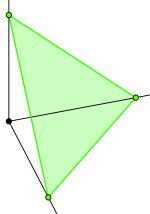
\includegraphics[scale=0.2]{simplex}
\caption{A simplex in R3 [8]}
\end{wrapfigure}
A portfolio of $n$ stocks denoted $a_1 , \dots , a_n$ can be represented as a sequence of weights $\pi_1, \dots , \pi_n$, where
\begin{equation}
\sum_{i=1}^n \pi_i =1; \quad 0 \leq \pi_i \leq 1 \forall i.
\end{equation}
Each weight $\pi_i$ corresponds to the proportion of the portfolio allocated to $a_i$. The set of all points satisfying these constraints, points in $\mathbb{R}^n$ whose coordinates sum to 1 and are individually bounded by 0 and 1, is an $n$-dimensional simplex, a hyperplane of $\mathbb{R}^n$ with some
special properties. In particular, simplexes are a focus of information geometry. Therefore, we can use an $n$-dimensional simplex to represent all possible portfolios of $n$ stocks.



\subsection{Portfolio Returns}
\begin{wrapfigure}{r}{0.3\textwidth}
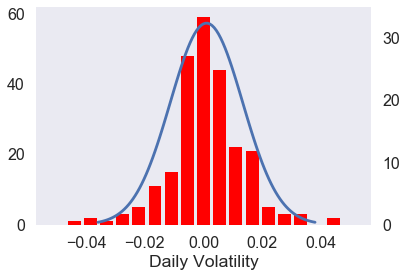
\includegraphics[scale=0.3]{aaplnormal}
\caption{The distribution of the log daily returns of AAPL overlaid with a normal distribution with matching standard deviation and mean}
\end{wrapfigure}
It has been empirically observed in the field of finance that asset returns follow a log normal distribution. That is, the logarithmic continuous growth rates of asset prices roughly fit a normal distribution, though in practice the distributions of returns tend to have thinner sides and fatter tails than normal distributions owing to the existence of news events such as earning reports that cause large, sudden shifts in asset prices. Figure 2 visually shows how well asset returns fits a normal distribution, in this case using the past year’s log daily returns for Apple stock.
To compute the log continuous growth rates for an asset,
we will look at the daily close of each asset $a_i$’s price (the
value of the asset at 4:00 PM ET, when markets close), divide it by the previous day's close, then take the logarithm
of that ratio. Once we have done so for every day in our
sample (we use the previous one year’s worth of data for every trading day), we take the mean, which gives us our expected daily return over the long run $\mu_i$. The standard deviation of the log returns gives us $\sigma_i$, which will act as our proxy for risk.
Once we have the expected return $\mu_i$ for each asset $a_i$ in our portfolio, the expected returns of the overall portfolio is simply a weighted sum of the returns of the individual assets
\begin{equation}
\mu_\pi = \sum_{i=1}^n \pi_i \mu_i = \pi \cdot \mu
\end{equation}



\subsection{Portfolio Risk}
The risk level of portfolio is slightly less straightforward, owing to the fact that the returns of different assets are correlated with one another. As such it is necessary to use the covariance between pairs of assets when calculating the risk of the portfolio overall. Let $R_i$ be the distribution of returns corresponding to asset $a_i$. Using the statistical formula for the risk of correlated distributions, we get
\[\sigma_\pi^2 \sum_{i,j=1}^n \sigma_\pi^2 = \pi_i \pi_j Cov(R_i,R_j),\]
where $Cov(Ri,Rj)$ is the covariance of the returns for assets $i$ and $j$ [1].  This is equivalent to the norm of the weight vector under the Mahalanobis metric, so we can equivalently compute the risk as
\begin{equation}
\sigma_\pi = \sqrt{\pi \cdot C\pi}
\end{equation}
where $C$ is the covariance matrix of the log returns of the assets.


\section{Sharpe Surface}


We'll define the Sharpe Surface as the range of the function $s: V \rightarrow \mathbb{R}$, where $V$ is the range set of all possible portfolio configurations, and $s$ is the function that calculates the Sharpe ratio of a portfolio.
For a portfolio vector $\pi\in V$, the Sharpe ratio associated with that vector is
\[s(\pi) = \frac{\pi \cdot \mu}{\sqrt{\pi \cdot C \pi}}\]
We'd like to know the gradient of this surface at a given point.  To obtain this, we take the partial derivative with respect to $\pi_i$ 
\[\frac{\partial s}{\partial \pi_i} = \frac{\pi_i \mu_i \sqrt{\pi \cdot C \pi} - \frac{ \pi \cdot \mu}{2\sqrt{\pi \cdot C \pi}}(\pi'\cdot C\pi + \pi \cdot C\pi') }{\pi \cdot C \pi}\]
%\newpage
%Now consider the second derivative with respect 
%\[\frac{\partial^2 s}{\partial \pi_i^2} = \frac{(\pi \cdot C \pi)[\mu_i \sqrt{\pi \cdot C \pi} + \frac{ \pi \cdot \mu}{2\sqrt{\pi \cdot C \pi}}(\pi'\cdot C\pi + \pi \cdot C\pi')
% - \frac{1}{2}\frac{\partial s}{\partial \pi_i} (\pi'\cdot C\pi + \pi \cdot C\pi') - \frac{ \pi \cdot \mu}{\sqrt{\pi \cdot C \pi}} \pi' \cdot C\pi']}{(\pi \cdot C \pi)^2}\]
%\[  - \frac{(\pi'\cdot C\pi + \pi \cdot C\pi')[\pi_i \mu_i \sqrt{\pi \cdot C \pi} - \frac{ \pi \cdot \mu}{2\sqrt{\pi \cdot C \pi}}(\pi'\cdot C\pi + \pi \cdot C\pi')]}{(\pi \cdot C \pi)^2}\]

%\[\frac{\partial^2 s}{\partial \pi_i^2} = \frac{(\pi \cdot C \pi)[\mu_i \sqrt{\pi \cdot C \pi} + \frac{ \pi \cdot \mu}{\sqrt{\pi \cdot C \pi}}(\pi'\cdot C\pi )
% - \frac{\partial s}{\partial \pi_i} (\pi'\cdot C\pi) - \frac{ \pi \cdot \mu}{\sqrt{\pi \cdot C \pi}} \pi' \cdot C\pi']}{(\pi \cdot C \pi)^2}\]
%\[  -2 \frac{(\pi'\cdot C\pi )[\pi_i \mu_i \sqrt{\pi \cdot C \pi} - \frac{ \pi \cdot \mu}{\sqrt{\pi \cdot C \pi}}(\pi'\cdot C\pi )]}{(\pi \cdot C \pi)^2}\]
%
%\newpage
where $\pi'$ is the derivative of $\pi$ with respect to $\pi_i$, i.e., a one-hot vector with a 1 in the $i$th place and zeros elsewhere.
For a portfolio with $n$ assets, there are only $n-1$ degrees of freedom, so we want the space of vectors which $\pi$ can come from to be $n-1$ dimensions instead of $n$.  To do so, consider the diffeomorphism $\phi : U \rightarrow V$
\[\phi(\pi_1, \pi_2, \dots, \pi_{n-1}) \mapsto (\pi_1, \pi_2, \dots, \pi_{n-1}, 1 - \pi_1 - \pi_2 - \dots - \pi_{n-1})\]
Note that the linearity of this map combined with the restriction that $\sum_{i=1}^n \pi_i = 1$ makes the map invertible, and the linearity makes the map and its inverse differentiable.
We now parametrize the Sharpe Surface by $\psi = s \circ \phi$.  For $\pi \in U$, we then get
\[\psi(\pi) = \frac{\phi(\pi) \cdot \mu}{\sqrt{\phi(\pi) \cdot C \phi(\pi)}} \]
as the new parametrization of our surface.

To account for the mapping from $U$ to $V$, we must establish a connection $\nabla :(U,V)\rightarrow \nabla_U V$.  This connection gets associated with a matrix.
Then the gradient in terms of a weight vector from $U$ becomes
\[\nabla \psi= D\phi [\frac{\pi_i \mu_i \sqrt{\phi(\pi) \cdot C \phi(\pi) } - \frac{ \phi(\pi)  \cdot \mu}{2\sqrt{\phi(\pi)  \cdot C \phi(\pi) }}(\pi'\cdot C \phi(\pi)  + \phi(\pi)  \cdot C\pi') }{\phi(\pi)  \cdot C \phi(\pi) }]\]
where the [] denote the vector formed by all values $1\leq i \leq n-1$, where $D\phi$ is the Jacobian matrix of $\phi$.  Since our function is the identity map in all but one element, $D\phi$ looks like an $(n-1)\times (n-1)$ identity matrix with an extra row full of $-1$ at the bottom.

\subsection{Convexity}
Let $f: X \rightarrow \mathbb{R}$ and $x_1, x_2 \in X$.  Let $[x_1, x_2]$ be the line segment from $x_1$ to $x_2$ and $g(x)$ be the line segment from $f(x_1)$ to $f(x_2)$ such that $g(x_1)=f(x_1)$ and $g(x_2)=f(x_2)$.
A function $f$ is convex if for any $x\in [x_1, x_2]$, $g(x) \geq f(x)$.  
Notice that if the opposite is true---$g(x) \leq f(x)$ for any $x\in [x_1, x_2]$---then $f(x)$ can be made convex by letting $h(x)=-f(x)$.  For our purposes, we will use this second definition.


Consider two portfolios $\pi_a$ and $\pi_b$.  Let $\alpha \in [0,1]$ and let $\pi_c = \alpha \pi_a + (1-\alpha)\pi_b$.  Note that since $\phi$ is a linear function, $\phi(\alpha \pi_a + (1-\alpha)\pi_b) = \alpha \phi(\pi_a) + (1-\alpha)\phi(\pi_b)$.
Now we'll calculate the Sharpe ratio for $\phi(pi_c)$.  For simplicity of notation, we'll just use $\pi$ instead of $\phi(\pi)$ for $\pi = \pi_a, \pi_b, \pi_c$.
\[s(\pi_c) = \frac{(\alpha \pi_a + (1-\alpha)\pi_b) \cdot \mu}{\sqrt{(\alpha \pi_a + (1-\alpha)\pi_b)\cdot C(\alpha \pi_a + (1-\alpha)\pi_b)}}\]
To show convexity, we wish to show that this value is greater than or equal to
\[\frac{\alpha \pi_a\cdot \mu }{\sqrt{\pi_a \cdot C \pi_a}} +\frac{ (1-\alpha) \pi_b\cdot \mu }{\sqrt{\pi_b \cdot C \pi_b}}\]


Since the terms in the square root represent norms under the Mahalanobis distance, they obey the triangle inequality.  Therefore the denominator of the Sharpe ratio is less than or equal to
\[\sqrt{\alpha \pi_a \cdot C\alpha \pi_a} +\sqrt{ (1-\alpha)\pi_b \cdot C(1-\alpha)\pi_b} = \alpha\sqrt{ \pi_a \cdot C \pi_a} +(1-\alpha) \sqrt{ \pi_b \cdot C\pi_b}\]
Therefore
\[s(\pi_c) \geq \frac{\alpha \pi_a \cdot \mu + (1-\alpha)\pi_b \cdot \mu}{\alpha\sqrt{ \pi_a \cdot C \pi_a} +(1-\alpha) \sqrt{ \pi_b \cdot C\pi_b}}\]


We can get common denominators by multiplying by convenient ones, then ignore the common denominators, leaving
\[(\alpha \pi_a \cdot \mu + (1-\alpha)\pi_b \cdot \mu)\sqrt{\pi_a \cdot C \pi_a}\sqrt{\pi_b \cdot C \pi_b}\]
for the Sharpe ratio and
\[(\alpha \pi_a \cdot \mu \sqrt{\pi_b \cdot C \pi_b} + (1-\alpha) \pi_b\cdot \mu \sqrt{\pi_a \cdot C \pi_a})\]
\[(\alpha\sqrt{ \pi_a \cdot C \pi_a} +(1-\alpha) \sqrt{ \pi_b \cdot C\pi_b})\]
for the point on the line segment.

The point on the line segment becomes
\[\alpha\pi_a \cdot \mu [\alpha \sqrt{\pi_b \cdot C \pi_b} \sqrt{\pi_a \cdot C \pi_a} + (1-\alpha) \pi_b \cdot C\pi_b ]+\]
\[(1-\alpha)\pi_b \cdot \mu [(1-\alpha) \sqrt{\pi_b \cdot C \pi_b} \sqrt{\pi_a \cdot C \pi_a} + \alpha \pi_a \cdot C\pi_a ]\]

To obtain the desired inequality, we need 
\[\alpha(1-\alpha)[(\pi_b \cdot \mu )\pi_a \cdot C\pi_a + ( \pi_a \cdot \mu )\pi_b \cdot C\pi_b ] \leq\]
\[\alpha(1-\alpha)(\pi_a \cdot \mu + \pi_b \cdot \mu)\sqrt{\pi_b \cdot C \pi_b} \sqrt{\pi_a \cdot C \pi_a} \]


This simplifies to
\[(\pi_b \cdot \mu )\pi_a \cdot C\pi_a + ( \pi_a \cdot \mu )\pi_b \cdot C\pi_b  \leq \]
\[(\pi_a \cdot \mu + \pi_b \cdot \mu)\sqrt{\pi_b \cdot C \pi_b} \sqrt{\pi_a \cdot C \pi_a} \]
Without loss of generality, let $\pi_b \cdot \mu > \pi_a \cdot \mu$.  Then this inequality holds if $\sqrt{\pi_b \cdot C \pi_b} > \sqrt{\pi_a \cdot C \pi_a}$, i.e. if portfolios with higher returns are riskier. 
%Manipulate both sides to
%\[(\pi_a \cdot \mu + \pi_b \cdot \mu)(\pi_a \cdot C\pi_a + \pi_b \cdot C\pi_b)  \leq \]
%\[(\pi_a \cdot \mu + \pi_b \cdot \mu)\sqrt{\pi_b \cdot C \pi_b} \sqrt{\pi_a \cdot C \pi_a} + \]\[(\pi_a \cdot \mu )\pi_a \cdot C\pi_a + (\pi_b \cdot \mu )\pi_b \cdot C\pi_b\]
%Which factors into
\subsection{Capital Asset Pricing Model}
The Capital Asset Pricing Model (CAPM) is a theory for asset return rate developed by Sharpe, Markowitz and Miller which jointly earned them a Nobel prize in economics.  Their theory indicates that the return rate of an asset varies directly with the risk of the asset.  Under these assumptions, the inequality $\sqrt{\pi_b \cdot C \pi_b} > \sqrt{\pi_a \cdot C \pi_a}$ holds true.  Therefore as long as the assets we choose obey the assumptions of CAPM, the resulting Sharpe surface will be convex.


\section{Methods} 
The methods section consists of both the gradient descent algorithm itself and the methods used to backtest the algorithm’s performance. The gradient descent algorithm is an alteration of stochastic gradient descent algorithms owing to the fact that rather than having a large set of sample inputs and target outputs, we instead have one target distribution and a single set of input stocks. As a result, rather than stochastically estimating the gradient, we directly compute the gradient of the Sharpe surface with respect to the portfolio weights. My backtesting approach rather simply applies the algorithm every day to compute new weights, invests based on that, and records the resulting change in portfolio value at the end of each day.



\subsection{Gradient Descent Algorithm}
To perform gradient descent over an error surface, at each point, we need to calculate the gradient with respect to the weights, then take a small step in the direction of most negative gradient. We do this until the error stops changing with successive steps, indicating a gradient of the zero vector, which indicates a minimum. Since the error surface has no global minima, this minimum must represent the portfolio weights with the least error.
To implement this algorithm, we must compute the gradient of the KL-divergence with respect to each portfolio weight $\pi_i$. Let $p$ be the distribution of log returns generated according to the portfolio weights and let q be the target distribution. Let $\mu_1$ and $\mu_2$ be the respective means and $\sigma_1$ and $\sigma_2$ be the respective standard deviations of p and q. Then we have

It’s straightforward to precompute the covariance matrix and expected returns for all of the assets’ returns ahead of time, so everything in this expression is in terms of readily available information, so this can be computed easily inside of an algorithm.
To perform gradient descent according to this rule, during each update step (also called training epoch), the weights are updated according to the following rule:
\[\pi_{t=k+1} = \pi_{t=k} - \epsilon\nabla [s(\pi_{t=k})],\]
Where $\pi_{t=k}$ is the portfolio weight vector after $k$ update iterations, $s$ is the function to calculate the Sharpe ratio of a portfolio, and $\nabla$ is the gradient operator with respect to each $\pi_i$.

However, after adding the adjustment term, our portfolio vector may no longer still lie on the simplex, as it may no longer satisfy the hyperplane equation
\[\pi_1 + \pi_2 + \dots + \pi_n = 1.\]
We wish to restore this property while staying as close to the current vector as possible, so we will use an orthogonal projection.  
To do so, we need to know the direction of the normal vector to the hyperplane.  For any hyperplane, a normal vector may be found by simply taking the coefficients of the vector components and putting them in a vector, then normalizing.  
Since all of our $n$ coefficients are $1$, our normal vector simply becomes an $n$-length vector with $\frac{1}{\sqrt{n}}$ in every location.  To scale this this to the proper to return our weight vector to the hyperplane, simply multiply the vector by $\frac{1}{\sqrt{n}}([\sum_{i=1}^n \pi_i] - 1)$, which will restore the size of the vector to 1.

We will also use a variable learning rate, which is a mechanism that gradient descent algorithms use to help them converge faster. 
The variable learning rate strategy we used is to increase $\epsilon$ by a factor of 1.05 whenever the most recent update caused the error to decrease and to decrease $\epsilon$ by a factor of 0.7 whenever the most recent update caused the error to increase by a factor of 1.04 or greater. 
My implementation of the algorithm used 800 training epochs and an initial learning rate of $\epsilon = 0.001$. These values were chosen through trial and error to get the algorithm to quickly and consistently converge.


\subsection{Backtesting}
I implemented by backtesting script in Python 3 in a Juptyer Notebook using data made available by iextrading.com. The stocks I considered investing in were 25 stocks chosen from the Dow Jones Industrial Average (DJIA). The five DJIA stocks I did not consider were excluded because my data source, Quandl.com, did not have enough of their historical pricing data freely available in order for me to include them in my testing1.
For each of the past 150 trading days\footnote{The stocks I excluded were 3M (MMM), Apple (AAPL), DowDuPont (DWDP), Intel (INTC), and Travelers Companies (TRV).}$^,$\footnote{Trading days are Mondays through Fridays excluding holidays. The last trading day I used in my testing was May 12, 2018.}, I ran the gradient descent algorithm on the previous year’s worth of data (251 trading days) to obtain the portfolio weights with the best Sharpe ratio.
I then calculated the returns that a portfolio with the determined weights would have had on that day and applied that rate of return to a portfolio with an initial value of \$10,000. For the sake of comparison, I also tracked the performance of the Dow Jones Industrial Average over that time period as a baseline, and applied that growth rate to a portfolio with an initial value of \$10,000.  I also implemented a version of the algorithm which can go short in assets by performing gradient descent twice---once in the fashion described above, and once where the asset return rates have been flipped to indicate going short.  The two portfolios are then combined, where the extra cash available from shorting the short asset are invested into the long portfolio at double the rate.

\section{Results}
\begin{figure}[h!]%{c}{0.3\textwidth}
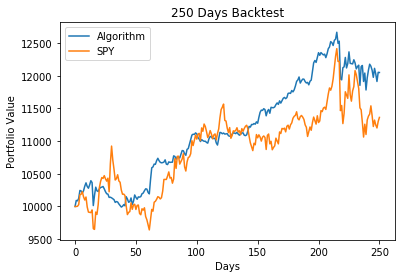
\includegraphics[scale=0.9]{back1}
\caption{Backtest over the past year's worth of trading days using a long-only portfolio}
\end{figure}

\begin{figure}[h!]%{c}{0.3\textwidth}
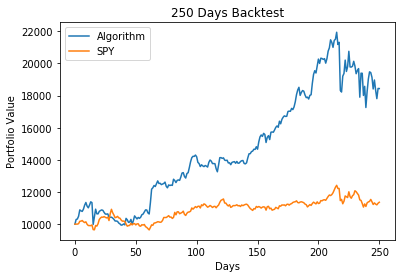
\includegraphics[scale=0.9]{back2}
\caption{Backtest over the past year's worth of trading days using a portfolio including shorts}
\end{figure}

In Figures 3 and 4 on the following page, the orange line represents the performance of \$10,000 invested in a SPY, an index ETF which tracks the performance of the S\&P 500, and the blue line represents the performance of \$10,000 invested according to the algorithm.  The market growth rate is typically considered to be a good benchmark for investment performance.

Over the course of 250 trading days, the long-only gradient descent algorithm resulted in a growth rate of 20.50\% compared with a growth of only 13.56\% for SPY.  Meanwhile, the porfolio which allows for shorting assets showed an 84.37\% increase over the same period of time.  Figures 3 and 4 show the performance of each algorithm relative to SPY, and Figure 5 shows both together.  We can visually observe in Figure 3 that the portfolio created by our algorithm was less volatile than the market and performed somewhat better.  Meanwhile, Figure 4 demonstrates that adding a short component substantially increased the growth rate by a great deal while also significantly increasing the volatility.

\begin{figure}[h!]%{c}{0.3\textwidth}
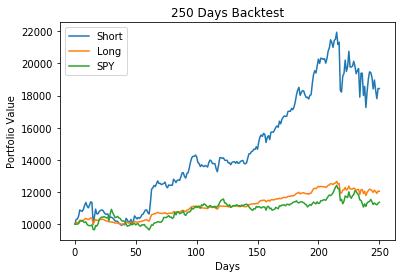
\includegraphics[scale=0.9]{back3}
\caption{Comparison of both algorithms to the market}
\end{figure}


\section{Future Work}
This algorithm demonstrates the gradient descent along an surface generated by the equation of the sharpe ratio is a promising approach for tackling problems in portfolio theory. There are several directions in which to expand this algorithm.
First, we could explore problems around portfolio selection, that is, determining which assets are best to include in the portfolio.
Another extension would be to study the rebalancing frequency. Out of convenience with respect to data availability, I used daily returns, hence optimizing the Sharpe ratio over a 1-day horizon, so I
rebalanced daily. It’s quite possible that this is not the optimal frequency with respect to long-term growth, and insight into this problem could be found in Wong’s thesis, which focused on rebalancing frequency [1].
There is also the possibility of exploring different risk metrics to use; I recently heard of a type of probability distribution called a Slash distribution, which has similar features to a normal distribution, but features the narrower sides and fatter tails which have been empirically observed in asset log growth rates.

\newpage
\section*{References}
[1] Wong, T. 2016, ’Geometry and Optimization of Relative Arbitrage’, PhD Thesis, University of Michigan, Ann Arbor MI.

[4] ‘NumPy Reference — NumPy v1.14 Manual’, Docs.scipy.org, \url{https://docs.scipy.org/doc/numpy/ reference/}

[5] ‘Matplotlib 2.2.0 documentation’, Matplotlib.org, \url{https://matplotlib.org/#documentation}

Data Sources:

[6] ‘IEX Trading’, IEXTrading.com, \url{https://www.iextrading.com/}

[7] ‘\^DJI Historical Prices | Dow Jones Industrial Average Stock - Yahoo Finance’, Finance.yahoo.com, \url{https://finance.yahoo.com/quote/\%5EDJI/history?p=\%5EDJI}
Image Sources:

[8] ‘Simplex’, Wikipedia.org, \url{https://en.wikipedia.org/wiki/Simplex}

[9] `Capital Asset Pricing Model', Wikipedia.org, \url{https://en.wikipedia.org/wiki/Capital_asset_pricing_model}

\end{document}
